%!TEX root = ../DSGEnotes.tex
\section{经验验证}
\label{sec:stylized-empirics}
结合前文提到的典型DSGE模型及其状态——空间表达形式,本节做经验验证。具体说来,截取美国1984Q1-2007Q4的季度经济数据作样本(对应从大调整时期之后, the Great Moderation到大衰退时间之前, the Great Recession period),模拟全体矩。


数据下载自FRED数据库(Federal Reserve Bank of St. Louis, https://fred.stlouisfed.org/),结合模型实际需要,包括以下诸项(表  \ref{tab:stylized-ssrep-empirics-data}):
\begin{itemize}
  \item 实际总产出(seasonally adjusted GDP at the annual rate, 2009 dollars). GDPC96.
  对季度产出取$\log$后相减。
  \item 劳动收入份额(seasonally adjusted GDP at the annual rate),计算方法为$\log \left(\frac{COE}{GDP}\right)$,COE表示compensation of employees.
  \item 通货膨胀率。implicit price deflator. GDPDEF. 对季度数据取$\log$后相减。
  \item 回报率。Effective Federal Funds Rate. GDPDEF. 是月度数据并且未经seasonally adjusted。将每个季度的三个月度数据取平均数,化为季度数据。
\end{itemize}


\begin{longtable}{p{.20\textwidth}|p{.20\textwidth}p{.20\textwidth}p{.20\textwidth}p{.20\textwidth}}
        \hline
        &$\log\left( X_{t}/X_{t-1} \right)$	&$\log (lsh_{t})$	& $ \pi_{t}$	& $R_{t}$\\
        \hline
        1984-01-01	&0.0197	&-0.7846	&0.0106	&0.0969\\
        1984-04-01	&0.0174	&-0.7866	&0.0084	&0.1056\\
        1984-07-01	&0.0098	&-0.7836	&0.0081	&0.1139\\
        1984-10-01	&0.0079	&-0.7808	&0.0067	&0.0927\\
        1985-01-01	&0.0099	&-0.7843	&0.0114	&0.0848\\
        1985-04-01	&0.0091	&-0.7844	&0.0062	&0.0792\\
        1985-07-01	&0.0154	&-0.7891	&0.0058	&0.0790\\
        1985-10-01	&0.0075	&-0.7820	&0.0058	&0.0810\\
        1986-01-01	&0.0092	&-0.7823	&0.0049	&0.0783\\
        1986-04-01	&0.0046	&-0.7821	&0.0040	&0.0692\\
        1986-07-01	&0.0100	&-0.7820	&0.0040	&0.0621\\
        1986-10-01	&0.0052	&-0.7737	&0.0056	&0.0627\\
        1987-01-01	&0.0070	&-0.7689	&0.0072	&0.0622\\
        1987-04-01	&0.0112	&-0.7703	&0.0067	&0.0665\\
        1987-07-01	&0.0090	&-0.7688	&0.0072	&0.0684\\
        1987-10-01	&0.0164	&-0.7673	&0.0082	&0.0692\\
        1988-01-01	&0.0056	&-0.7653	&0.0078	&0.0666\\
        1988-04-01	&0.0131	&-0.7651	&0.0096	&0.0716\\
        1988-07-01	&0.0058	&-0.7659	&0.0117	&0.0798\\
        1988-10-01	&0.0132	&-0.7694	&0.0080	&0.0847\\
        1989-01-01	&0.0100	&-0.7763	&0.0109	&0.0944\\
        1989-04-01	&0.0078	&-0.7860	&0.0103	&0.0973\\
        1989-07-01	&0.0074	&-0.7896	&0.0072	&0.0908\\
        1989-10-01	&0.0021	&-0.7822	&0.0069	&0.0861\\
        1990-01-01	&0.0109	&-0.7842	&0.0110	&0.0825\\
        1990-04-01	&0.0039	&-0.7803	&0.0103	&0.0824\\
        1990-07-01	&0.0002	&-0.7775	&0.0089	&0.0816\\
        1990-10-01	&-0.0086	&-0.7747	&0.0075	&0.0774\\
        1991-01-01	&-0.0047	&-0.7790	&0.0099	&0.0643\\
        1991-04-01	&0.0077	&-0.7844	&0.0068	&0.0586\\
        1991-07-01	&0.0048	&-0.7875	&0.0073	&0.0564\\
        1992-01-01	&0.0117	&-0.7829	&0.0043	&0.0402\\
        1991-10-01	&0.0044	&-0.7873	&0.0054	&0.0482\\
        1992-04-01	&0.0110	&-0.7869	&0.0064	&0.0377\\
        1992-07-01	&0.0097	&-0.7935	&0.0047	&0.0326\\
        1992-10-01	&0.0100	&-0.7955	&0.0067	&0.0304\\
        1993-01-01	&0.0019	&-0.8035	&0.0057	&0.0304\\
        1993-07-01	&0.0049	&-0.8018	&0.0060	&0.0306\\
        1993-04-01	&0.0059	&-0.8000	&0.0061	&0.0300\\
        1993-10-01	&0.0133	&-0.8052	&0.0052	&0.0299\\
        1994-01-01	&0.0098	&-0.8156	&0.0048	&0.0321\\
        1994-04-01	&0.0136	&-0.8117	&0.0050	&0.0394\\
        1994-07-01	&0.0059	&-0.8127	&0.0054	&0.0449\\
        1994-10-01	&0.0113	&-0.8133	&0.0055	&0.0517\\
        1995-01-01	&0.0034	&-0.8076	&0.0057	&0.0581\\
        1995-04-01	&0.0035	&-0.8052	&0.0044	&0.0602\\
        1995-07-01	&0.0085	&-0.8059	&0.0047	&0.0580\\
        1995-10-01	&0.0071	&-0.8064	&0.0049	&0.0572\\
        1996-01-01	&0.0065	&-0.8048	&0.0054	&0.0536\\
        1996-04-01	&0.0173	&-0.8076	&0.0038	&0.0524\\
        1996-07-01	&0.0092	&-0.8042	&0.0028	&0.0531\\
        1996-10-01	&0.0105	&-0.8044	&0.0051	&0.0528\\
        1997-01-01	&0.0076	&-0.7984	&0.0062	&0.0528\\
        1997-04-01	&0.0150	&-0.8007	&0.0027	&0.0552\\
        1997-07-01	&0.0127	&-0.7993	&0.0036	&0.0553\\
        1997-10-01	&0.0077	&-0.7883	&0.0033	&0.0551\\
        1998-01-01	&0.0098	&-0.7786	&0.0016	&0.0552\\
        1998-04-01	&0.0097	&-0.7734	&0.0021	&0.0550\\
        1998-07-01	&0.0130	&-0.7732	&0.0037	&0.0553\\
        1998-10-01	&0.0163	&-0.7760	&0.0031	&0.0486\\
        1999-01-01	&0.0080	&-0.7696	&0.0050	&0.0473\\
        1999-04-01	&0.0082	&-0.7716	&0.0033	&0.0475\\
        1999-07-01	&0.0125	&-0.7740	&0.0036	&0.0509\\
        1999-10-01	&0.0172	&-0.7718	&0.0046	&0.0531\\
        2000-01-01	&0.0029	&-0.7456	&0.0076	&0.0568\\
        2000-04-01	&0.0187	&-0.7642	&0.0057	&0.0627\\
        2000-07-01	&0.0012	&-0.7527	&0.0065	&0.0652\\
        2000-10-01	&0.0057	&-0.7586	&0.0054	&0.0647\\
        2001-01-01	&-0.0028	&-0.7447	&0.0063	&0.0559\\
        2001-04-01	&0.0053	&-0.7609	&0.0070	&0.0433\\
        2001-07-01	&-0.0032	&-0.7664	&0.0033	&0.0350\\
        2001-10-01	&0.0028	&-0.7726	&0.0030	&0.0213\\
        2002-01-01	&0.0092	&-0.7813	&0.0032	&0.0173\\
        2002-04-01	&0.0055	&-0.7808	&0.0037	&0.0175\\
        2002-07-01	&0.0049	&-0.7881	&0.0044	&0.0174\\
        2002-10-01	&0.0006	&-0.7920	&0.0054	&0.0144\\
        2003-01-01	&0.0052	&-0.8013	&0.0061	&0.0125\\
        2003-04-01	&0.0092	&-0.7998	&0.0032	&0.0125\\
        2003-07-01	&0.0166	&-0.8093	&0.0055	&0.0102\\
        2003-10-01	&0.0116	&-0.8094	&0.0047	&0.0100\\
        2004-01-01	&0.0057	&-0.8181	&0.0087	&0.0100\\
        2004-04-01	&0.0073	&-0.8148	&0.0087	&0.0101\\
        2004-07-01	&0.0090	&-0.8101	&0.0061	&0.0143\\
        2004-10-01	&0.0086	&-0.8186	&0.0070	&0.0195\\
        2005-01-01	&0.0106	&-0.8294	&0.0092	&0.0247\\
        2005-04-01	&0.0052	&-0.8312	&0.0072	&0.0294\\
        2005-07-01	&0.0084	&-0.8317	&0.0093	&0.0346\\
        2005-10-01	&0.0057	&-0.8322	&0.0076	&0.0398\\
        2006-01-01	&0.0119	&-0.8240	&0.0078	&0.0446\\
        2006-04-01	&0.0030	&-0.8285	&0.0080	&0.0491\\
        2006-07-01	&0.0009	&-0.8288	&0.0070	&0.0525\\
        2006-10-01	&0.0078	&-0.8210	&0.0035	&0.0525\\
        2007-01-01	&0.0006	&-0.8058	&0.0112	&0.0526\\
        2007-04-01	&0.0076	&-0.8153	&0.0056	&0.0525\\
        2007-07-01	&0.0067	&-0.8220	&0.0035	&0.0507\\
        2007-10-01	&0.0036	&-0.8183	&0.0043	&0.0450\\
        \hline
%        \centering
      \caption{用于经验验证的观测数据集}

      \small{数据来源:FRED database. 整理后放在\textit{./data/20180403-empirics.xlsx} 中。}
        \label{tab:stylized-ssrep-empirics-data}
\end{longtable}

\subsection{自协方差}
\label{sec:stylized-ssrep-empirics-var}

我们计算样本的协方差$\widehat{\Gamma}_{yy} \left(h \right)$,作为全体自协方差$\Gamma_{yy} \left(h \right)$的近似
\begin{equation}
  \label{eq:stylized-ssrep-empirics-autocovar}
  \widehat{\Gamma}_{yy} \left( h \right) = \frac{1}{T}
  \sum_{t=h}^{T} \left( y_{t} - \hat{\mu}_{y} \right) \,
  \left( y_{t} - \hat{\mu}_{y} \right)^{\top}, \quad \, \mu_{y} = \frac{1}{T} \sum_{t=1}^{T} y_{t}.
\end{equation}

在满足一定的正则条件的前提下,根据强大数法则(strong law of large numbers, SSLN, 第\ref{sec:lln-slln}节)和中心极限定理(central limit theorem, CLT,第\ref{sec:kernel-gaussian-central-limit-theorem}节)样本自协方差,$\widehat{\Gamma}_{yy} \left(h \right)$收敛至全体自协方差$\Gamma_{yy} \left(h \right)$,这些正则条件包括
\begin{itemize}
  \item 向量过程$y_{t}$的协方差是平稳的,
  \item $y_{t}$的序列相关的衰减速度足够快,
  \item $y_{t}$的(至少一系列)高阶矩是有界的,等。
\end{itemize}

如果研究目标包括计算自协方差矩阵的数列\footnote{Matlab中可用xcov程序计算自协方差、跨协方差。},一个比较有效率的求解方法是,首先建立一个辅助模型并作参数估计。第二步,将这个辅助模型的估计参数转换为自协方差数列的参数值。辅助模型有许多种类,一个较为合适的种类是线性向量自回归模型(Vector AutoregRessions, VARs)\index{VAR!(vector autoregression) \dotfill 向量自回归},一个简单的VAR(1)可表示如下
\begin{equation}
  \label{sec:stylized-ssrep-empirics-var1-def}
  y_{t} = \phi_{1} y_{t-1} + \phi_{0} + u_{t}, \quad u_{t} \sim i.i.d. \, \mathbb{N} \left(0, \Sigma \right),
\end{equation}
其中全体的OLS系数$\phi_{1}$向量,和残差方差$\Sigma$无法直接计算求得,可用样本的对应值$\hat{\phi}_{1}, \widehat{\Sigma}$予以近似,计算方法如下
\begin{align}
  \label{sec:stylized-ssrep-empirics-VAR1-sample-coef-phi1}
  \hat{\phi}_{1} & = \widehat{\Gamma}_{yy} \left( 1 \right)
  \widehat{\Gamma}_{yy}^{-1} \left( 0 \right) + \mathcal{O}_{p} \left( T ^{-1} \right), \\
  \label{sec:stylized-ssrep-empirics-VAR1-sample-coef-resvar}
  \widehat{\Sigma} & = \widehat{\Gamma}_{yy} \left( 0 \right)
  - \widehat{\Gamma}_{yy} \left( 1 \right)
  \widehat{\Gamma}_{yy}^{-1} \left( 0 \right)
  \widehat{\Gamma}_{yy}^{\top} \left( 1 \right)
  + \mathcal{O}_{p} \left( T ^{-1} \right),
\end{align}
其中$\mathcal{O}_{p} \left( T^{-1} \right)$用于反映OLS定义式的系数估计方法,和样本自协方差求和估计式\eqref{eq:stylized-ssrep-empirics-autocovar}之间的微小不一致——对于一组随机变量的数列$X_{t}$,如果随着$T \mapsto \infty$, $T X_{T}$随机有界,我们将数列$X_{t}$表示为$\mathcal{O}_{p} \left( T^{-1} \right)$。

$VAR(1)$过程的自协方差、跨协方差方程,类似于\eqref{eq:stylized-ssrep-autocov},分别表示为$\widehat{\Gamma}_{yy}^{V}(h),\, \widehat{\Gamma}_{ss}^{V}(h), \, \widehat{\Gamma}_{ys}^{V}(h)$,并且$\widehat{\Gamma}_{yy}(0)$和$\widehat{\Gamma}_{yy}(h)$
的计算方式,类似于\eqref{eq:stylized-ssrep-lyapunov-func}\eqref{eq:stylized-ssrep-cov-ss-h};将$\hat{\phi}_{1}$的近似估计\eqref{sec:stylized-ssrep-empirics-VAR1-sample-coef-phi1}插入到估计过程中去,有
\begin{align}
  \label{eq:stylized-ssrep-var1-autocov-yy0}
  \widehat{\Gamma}_{yy}^{V} \left( 0 \right) = & \widehat{\Gamma}_{yy} \left( 0 \right) + \mathcal{O}_{p} \left( T^{-1} \right), \\
  \label{eq:stylized-ssrep-var1-autocov-yyh}
  \widehat{\Gamma}_{yy}^{V} \left( h \right) = &
  \left( \hat{\phi}_{1} \right)^{h} \widehat{\Gamma}_{yy}^{V} \left( 0 \right) + \mathcal{O}_{p} \left( T^{-1} \right)
  = \left[ \widehat{\Gamma}_{yy} \left( 1 \right) \,
  \widehat{\Gamma}_{yy}^{-1} \left( 0 \right)
  \right]^{h}
  \widehat{\Gamma}_{yy} \left( 0 \right)
  + \mathcal{O}_{p} \left( T^{-1} \right).
\end{align}

来比较$\widehat{\Gamma}_{yy}^{V} \left( h \right)$和$\widehat{\Gamma}_{yy} \left( h \right)$:
\begin{equation*}
  \widehat{\Gamma}_{yy}^{V} \left( h \right) =
  \begin{cases}
    \widehat{\Gamma}_{yy} \left( h \right) + \mathcal{O}_{p} \left( T^{-1} \right) & h=0, \\
    \widehat{\Gamma}_{yy} \left( h \right) + \mathcal{O}_{p} \left( T^{-1} \right) & h=1, \\
    \left[ \widehat{\Gamma}_{yy} \left( 1 \right) \,
    \widehat{\Gamma}_{yy}^{-1} \left( 0 \right)
    \right]^{h}
    \widehat{\Gamma}_{yy} \left( 0 \right)
    + \mathcal{O}_{p} \left( T^{-1} \right) & h > 1,
  \end{cases}
\end{equation*}
换句话说,当$h=0,1$时两个自协方差的估计矩阵相等(除了$\mathcal{O}_{p} \left( T^{-1} \right)$的部分);而当$h>1$时二者不相等。\cite{Schorfheide:2005jg}指出,如果实际时间序列数据能够较好契合VAR(1)特征,那么插入法的估计$\widehat{\Gamma}_{yy}^{V} \left( h \right)$要比OLS估计$\widehat{\Gamma}_{yy} \left( h \right)$更有效。

实际研究过程中,有时时间序列数据并不符合VAR(1)特征。就需要在$VAR(p), \, p >1$框架下分析协自协方差
\begin{equation}
  \label{eq:stylized-ssrep-empirics-varp-def}
  y_{t} = \phi_{1} y_{t-1} + \ldots + \phi_{p} y_{t-p} + \phi_{0} + u_{t}, \quad \, u_{t} \sim i.i.d. \, \mathbb{N} \left( 0, \Sigma \right)
\end{equation}

$p$值的选取标准,可通过贝叶斯信息量(Bayesian information criterion, BIC)\index{Bayesian information criterion(BIC) \dotfill 贝叶斯信息量}方法予以估计。此外还有如赤池信息量(Akaike information criterion, AIC)\index{Akaike information criterion(AIC) \dotfill 赤池信息量}等方法。一个直观的处理方法是改写成友矩阵(companion matrix)形式,即将$VAR(p)$时间序列向量$y_{t}$理解为一个关于堆栈向量$\tilde{y}_{t} = \left[ y_{t}^{\top}, y_{t-1}^{\top}, \ldots, y_{t-p+1}^{\top} \right]$的$VAR(1)$过程:
\begin{equation}
  \label{sec:stylized-ssrep-empirics-varp-companion}
\begin{split}
    & \tilde{y}_{t} = \tilde{\phi}_{1} \tilde{y}_{t-1} + \tilde{\phi}_{0} + \tilde{u}_{t}, \quad \tilde{u}_{t} \sim \, i.i.d. \, \mathbb{N} \left( 0, \widetilde{\Sigma} \right),\\
    & \tilde{\phi_{1}} =
    \begin{pmatrix}
    \phi_{1} & \ldots & \phi_{p-1} & \phi_{p} \\
    I_{n \times n} & \ldots & 0_{n \times n} & 0_{n \times n} \\
    \vdots & \ddots & \vdots & \vdots \\
    0_{n \times n} & \ldots & I_{n \times n} & 0_{n \times n}
  \end{pmatrix},
  \quad \tilde{\phi}_{0} =
  \begin{pmatrix}
  \phi_{0} \\
  0_{n \left( p - n \right) \times 1}
  \end{pmatrix}, \\
  & \tilde{\epsilon_{t}} =
  \begin{pmatrix}
    \epsilon_{t} \\
    0_{n \left( p - n \right) \times 1}
  \end{pmatrix},
  \quad \widetilde{\Sigma} =
  \begin{pmatrix}
    \Sigma & 0_{n \times n \left( p - 1 \right)} \\
    0_{n \left( p - 1 \right) \times n} &
    0_{n \left( p - 1 \right) \times n \left( p - 1 \right)}
  \end{pmatrix},
\end{split}
\end{equation}
这样一来,估计的步骤如下:首先利用类似于\eqref{eq:stylized-ssrep-var1-autocov-yy0}\eqref{eq:stylized-ssrep-var1-autocov-yyh}的思路,将$y_{t}$替换为$\tilde{y}_{t}$,算得$\tilde{y}_{t}$的自协方差$\widehat{\Gamma}_{\widetilde{yy}}(0), \widehat{\Gamma}_{\widetilde{yy}}(h)$。
随后根据$y_{t} = M^{\top} \tilde{y}_{t}$,还原$y_{t}$的自协方差矩阵,其中$M^{\top}$是一个选择矩阵(selection matrix)\index{selection matrix \dotfill 选择矩阵}
\begin{equation*}
  M^{\top} = \left[ I_{n}, 0_{n \times n \left( p - 1 \right)}\right].
\end{equation*}

\begin{figure}[htbp]
  \caption{抽样观测数据的跨相关}
  \centering
  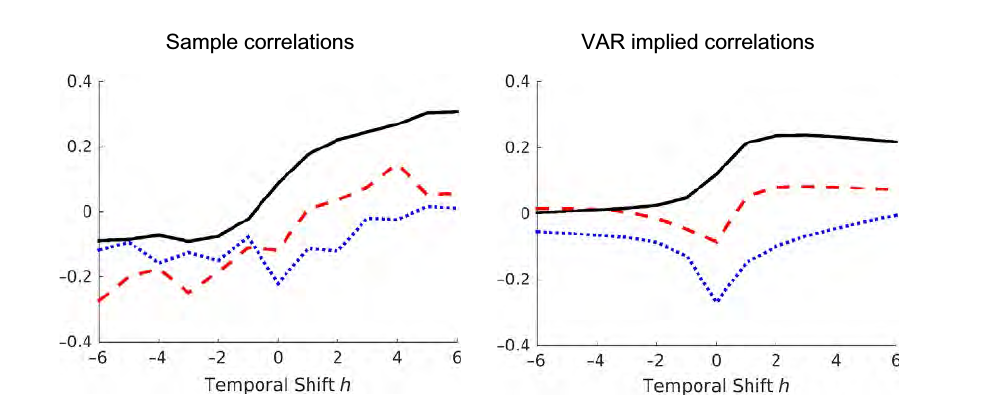
\includegraphics[width=12cm]{./Figures/20180404-corss-correlations}
  \label{fig:stylized-ssrep-cross-correlation}
%
%  \small{Source: PBOC.}
\end{figure}

图\eqref{fig:stylized-ssrep-cross-correlation}
画出了基于抽样观测数据(表\ref{tab:stylized-ssrep-empirics-data})的产出增速相对于利率(黑色实线),通货膨胀率(红色段线),劳动收入份额(蓝色点线)的跨相关(cross correlation)值\footnote{Matlab中用xcov计算,跨协方差就是跨相关方程。},横轴表示跨越的时间期$h$。左图使用样本自协方差矩阵$\widehat{\Gamma}_{yy} \left( h \right)$\eqref{eq:stylized-ssrep-empirics-autocovar}测算。右图使用$VAR(1)$测算而得\footnote{Matlab中用varm来作VAR分析。},其中其中根据BIC检验确定$p=1$,根据\eqref{eq:stylized-ssrep-empirics-autocovar}确定自协方差$\widehat{\Gamma}_{yy} \left( h \right)$。两组跨相关性质接近,但量化值不同,这是因为VAR模型更"吝啬"一些,导致VAR生成的相关系数更加平滑。

\subsection{光谱分析}
\label{sec:stylized-ssrep-empirics-spectral}
光谱分析的目标是近似计算光谱密度方程。
\subsubsection{样本平滑周期图法}
\label{sec:stylized-ssrep-empirics-spectral-direct}
直观上来看,对于常见的$VAR(1)$数列,我们似乎很容易用样本的周期图(periodgram)\index{periodgram \dotfill 周期图}来做光谱密度的近似估计,由\eqref{eq:stylized-ssrep-autocovariance-density}得
\begin{equation}
  \label{eq:spectral-periodgram-def}
\begin{split}
  \hat{f}_{yy} \left( \omega \right)
  & = \frac{1}{2 \pi} \sum_{h=-T+1}^{T-1} \widehat{\Gamma} \left( h \right)  \\
  & = \frac{1}{ 2 \pi}
  \left\{
  \widehat{\Gamma}_{yy} \left( 0 \right)
  + \sum_{h=1}^{T-1}
  \left[
  \widehat{\Gamma}_{yy} \left( h \right)
  + \widehat{\Gamma}_{yy}^{\top} \left( h \right)
  \right]
  \cos \left( \omega h \right)
  \right\},
\end{split}
\end{equation}
然而需要指出的是,尽管样本周期图对应的光谱密度 $\hat{f}_{yy} \left( \omega \right)$是对全体密度$f_{yy} \left( \omega \right)$的渐进无偏估计,但它并不适合用作近似估计,因为它不一致\footnote{
一致性(consistency)是指随着$T \rightarrow \infty$,估计值的偏差(biase)和方差都收敛至$0$,可参考\cite[Sec. 8.2]{Koopmans:1995vn}。}。

为了求得一致估计,需要沿着临近频率(adjacent frequencies)对样本周期图作平滑。基于基准频率(base frequency) $\omega = \frac{2 \pi}{T}$,定义一组基本频率(fundamental frequencies) $\left\{ \omega_{j} \right\}$,是基准频率的整数倍:
\begin{equation*}
  \omega_{j} = j \frac{2 \pi}{T}, \quad j = 1, \ldots, \frac{T-1}{2},
\end{equation*}

那么可以将平滑的周期图表示为$\overline{f}_{yy} \left( \omega \right)$,满足如下关系
\begin{equation}
  \label{eq:spectral-periodgram-smooth}
  \overline{f}_{yy} \left( \omega \right)  =
  \frac{\pi}{ \lambda \frac{T-1}{2}} \sum_{j=1}^{\frac{T-1}{2}}
  \mathcal{K} \left( \frac{\omega_{j} - \omega}{\lambda} \right)
  \hat{f}_{yy} \left( \omega_{j} \right),
\end{equation}
其中$\mathcal{K}(\cdot)$是一个核方程(kernel)\index{kernel \dotfill 核},满足$\int \mathcal{K}(x) \, \mathrm{d} x = 1$。核方程的具体形式有多种,一个简单的定义式可以表示为
\begin{equation}
  \label{eq:spectral-periodgram-smooth-kernel-def}
  \mathcal{K} \left( \frac{\omega_{j} - \omega}{\lambda} \right)
  \hat{f}_{yy} \left( \omega_{j} \right)
  \coloneqq \mathbb{I}
  \left\{
  - \frac{1}{2} < \frac{\omega_{j} - \omega }{\lambda} < \frac{1}{2}
  \right\}
  = \mathbb{I}
  \left\{
    \omega_{j} \in
    \mathbb{B} \left( \omega | \lambda \right)
  \right\},
\end{equation}
其中$\mathbb{I} \left\{ \cdot \right\}$是一个指示方程(indicator function)\index{indicator function \dotfill 指示方程}
见\eqref{eq:euler-complex-indicator-function-def},$\mathbb{B} \left( \omega | \lambda \right) = \lambda T \left( 2 \pi \right)$构成一个频率带(frequency band)\index{frequency band \dotfill 频率带}。关于核方程的简要介绍,可参考第\ref{sec:kernel-analysis}节。

如果有$\lim_{T \rightarrow \infty} \lambda \rightarrow 0$,即随着$T \rightarrow \infty$,频率的带宽缩减至$0$,那么对应地,$\mathbb{B} \left( \omega | \lambda \right)$中$\omega_{j}$的数量增大到无穷,平滑周期图算子因而是一致估计算子。

在经验研究中常常使用高斯核方程如$\exp \left( i \omega t \right)$作基方程(第\ref{sec:gaussian-kernel-fourier}节),从而$\mathcal{K}(x)$的值等于一个标准正态分布的随机变量的密度分布方程。

\subsubsection{VAR(p)的插入估值法}
\label{sec:stylized-ssrep-empirics-spectral-indirect}
若BIC检验结果表明观测数据更适合用VAR(p), $p >1$模型如\eqref{eq:stylized-ssrep-empirics-varp-def},那么可利用上文提到的插入法来近似估计光谱密度。具体说来,定义全体的系数向量$\phi \coloneqq \left[ \phi_{0}, \phi_{1}, \ldots, \phi_{p} \right]^{\top}$,选择矩阵$M(z) = \left[ Iz, \ldots, Iz^{p}\right]$。设样本的近似系数向量$\hat{\phi}$是对$\phi$的一个估计。

对应于VAR(1)下的\eqref{eq:stylized-ssrep-autocovariance-density-ss},VAR(p)用插入法估计的光谱分布密度$\hat{f}_{yy}^{V} \left( \omega \right)$可表示为
\begin{equation}
  \label{eq:stylized-ssrep-empirics-spectral-varp-plugin}
  \hat{f}_{yy}^{V} \left( \omega \right)
  = \frac{1}{2 \pi}
  \left[
  I - \hat{\phi}^{\top} M^{\top} \left( \exp \left( - i \omega \right) \right]
  \right]^{-1}  \hat{\Sigma} \,
  \left[
  I - M \left( \exp \left( - i \omega \right)  \right) \,\hat{\phi}
  \right]^{-1},
\end{equation}
\eqref{eq:stylized-ssrep-empirics-spectral-varp-plugin}是
对\eqref{eq:stylized-ssrep-autocovariance-density-ss}的一般化处理,将VAR(1)扩展到了VAR(p)的情况。

\begin{figure}[htbp]
  \caption{抽样数据的光谱分布密度}
  \centering
  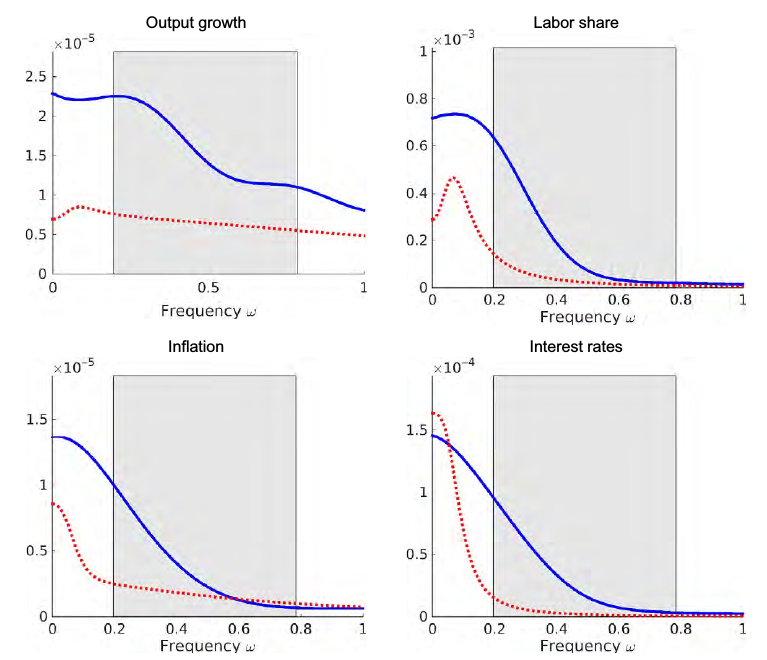
\includegraphics[width=12cm]{./Figures/20180406-empirics-spectrum}
  \label{fig:stylized-ssrep-empirics-spectrum}
%
%  \small{Source: PBOC.}
\end{figure}

图\ref{fig:stylized-ssrep-empirics-spectrum}依次绘出产出增速、劳动力收入份额、通货膨胀率和利率的光谱密度。阴影的矩形对应经济周期的频率$\left[ 0.196,0.785 \right]$。
红色点线表示根据$VAR(1)$ \eqref{eq:stylized-ssrep-autocovariance-density-ss}近似估计算得的密度分布,蓝色实线是根据高斯核方程$G \left(\cdot ; \sigma=0.15 \right)$ \eqref{eq:spectral-periodgram-smooth}算得的平滑周期图。

\begin{enumerate}
  \item 红色点线的光谱密度分布:
\begin{enumerate}
  \item 左上图:由于产出增速的自相关接近于$0$,使得光谱密度相对平缓。其余3张图中,三个观测数列在低频$\omega$处的光谱密度较高,这反映了实值域中三个时间序列具有较高的持久性。
  \item 劳动收入份额的光谱密度表现出明显的驼峰形,通胀和利率的的光谱密度随着频率$\omega$的增加而单调递减。
\end{enumerate}
\item 蓝色实线的平滑周期图分布:
\begin{enumerate}
  \item 对$\overline{f}_{yy} \left( \omega \right)$的估计值取决于带宽值的设定。我们在高斯方程中设$\sigma = 0.15$,大致说来在傅里叶域中,这对应于将样本周期图以约0.6的频带值做平均。
  \end{enumerate}
\end{enumerate}

\subsection{冲击响应方程}
\label{sec:stylized-ssrep-empirics-irfs}

VAR(p) \eqref{eq:stylized-ssrep-empirics-varp-def}有时也被称作缩减式VAR(reduced-form VAR)\index{VAR!reduced form \dotfill 缩减式向量自回归},这是由于新息向量$u_{t} \sim \, i.i.d. \, \mathbb{N} \left( 0, \Sigma \right)$并没有明确的结构性含义,它仅仅是前一时期的预测误差。

根据DSGE模型的设定,所谓冲击响应机制,是指某些新息冲击以结构性的方式作用于经济系统,使得经济系统做出响应,表现为同期系统模拟数据和现实观测数据之间的误差,即预测误差。可见,为了将基于VAR的冲击——响应(观测数据)和DSGE模型的冲击——响应(模拟数据)联系起来,就需要将预测误差引入到一个结构新息向量$\epsilon_{t}$中,设满足关系
\begin{equation}
  \label{eq:stylized-ssrep-svar-forecast-error}
  u_{t} = \phi_{\epsilon} \epsilon_{t} = \Sigma_{tr} \, \Omega \, \epsilon_{t},
\end{equation}
其中
\begin{itemize}
\item 对预测误差$u_{t}$的协方差矩阵$\Sigma$作Cholesky因式分解(Cholesky factorization,第\ref{sec:numlin-factorization-cholesky}节)\index{factorization!Cholesky \dotfill Cholesky因式分解},所生成的唯一的(对角元素非负)下三角矩阵,定义为$\Sigma_{tr}$,
\item $\Omega$是一个$n \times n$正交矩阵(orthogonal matrix,第\ref{sec:numlin-matrix-orthogonality}节)\index{matrix!orthogonal \dotfill 正交矩阵},满足
\begin{equation*}
  \Omega \, \Omega^{\top} = I.
\end{equation*}
\end{itemize}

引入$\Omega$的正交矩阵设定,是为了确保在状态——空间表现形式中,新息系数矩阵$\phi_{\epsilon}$可以写为如下关于$\Omega, \, \Sigma$的形式
\begin{equation}
  \label{eq:stylized-ssrep-svar-errorcoef-varcov}
  \phi_{\epsilon} \phi_{\epsilon}^{\top} = \Sigma_{tr} \, \Omega \, \Omega^{\top} \, \Sigma^{\top} = \Sigma.
\end{equation}
这样的向量自回归模型,我们称为结构向量自回归模型SVARs (structural vector autoregressions)\index{VAR!SVAR \dotfill 结构向量自回归}。
根据这样的架构设定,预测误差$u_{t}$的协方差矩阵$\Sigma$,与正交矩阵$\Omega$的具体选取无关。这意味着我们无法通过实际数据求得$\Omega$。大多数基于SVARs的研究文献仅仅对$\Omega$的设定做出必要的限定(restrictions),或称之为识别(identification)。随着冲击类型的不同(如技术进步,货币政策,公共支出等),附着在冲击上的新息也具有不同的性质,在构建模型时对应的限定/识别策略也有所区别,更详尽的综述可参考如\cite{Cochrane:1994gi, Christiano:1999uw, Stock:2001bp}等。

在(利用缩减式VAR)算得样本系数矩阵$\hat{\phi}$和$\hat{\Sigma}$的近似估计,以及明确对$\Omega$中一列或多列的识别机制之后,我们可以将样本近似下的冲击响应方程表示如下
\begin{equation}
  \label{eq:stylized-ssrep-sample-irfs}
  \widehat{IRF}^{V} \left( \cdot , j, h\right)
  = C_h \left( \hat{\phi} \right) \, \hat{\Sigma_{tr}} \, \left[ \Omega \right]_{.j},
\end{equation}
其中
\begin{itemize}
  \item $C_h \left( \hat{\phi} \right)$是移动平均系数矩阵(moving average coefficient matrix),可以通过VAR表现式\eqref{sec:stylized-ssrep-empirics-varp-companion}而算得
  \begin{equation}
    \label{eq:stylized-ssrep-sample-irfs-macoef}
    C_h \left( \hat{\phi} \right) = M^{\top} \, \widetilde{\phi}_{1}^{h} \, M, \quad \, M^{\top} \equiv \left[ I_{n}, 0_{n \times n \left( p - 1 \right)} \right].
  \end{equation}
  \item $\left[ \mathcal{A} \right]_{.j}$表示矩阵$\mathcal{A}$的第$j$列。
\end{itemize}

以下对IRFs的冲击——响应机制作一个响应区间的分析,即我们关注的是响应的方向(符号为正或为负),而非某一特定的数值,又称符号限制条件(sign restrictions)。这方面的研究可参考如\cite{Faust:1998be,Canova:2002hp,Uhlig:2005ks}等,它们将矩阵$\Omega$限定在一个有限的集合区间$\mathcal{O} \left( \phi, \sigma \right)$内,对应的IRFs需要满足该限定条件:只有在集合区间内的IRFs才被识别。

通过使用对数形式的产出增速、劳动收入份额,通货膨胀率和利率的VAR(1),我们可以将这个限定条件设为:面对一个紧缩型货币政策的点冲击,模型状态变量的响应表现为,在随后4个季度中通货膨胀率降低,利率上升。此外还做了一个不影响通用性的假定:将货币政策的冲击设为向量$q$(带宽),排在$\Omega$的第一列,用于描述冲击的效果。利用缩减式VAR估计得到的$\hat{\phi}, \, \hat{\Sigma}$,我们列出满足符号限定条件的IRFs集合,以确定单位长度向量$q$的集合,作为带宽。
\begin{figure}[htbp]
  \caption{冲击响应方程}\small{紧缩性货币政策冲击表现为$1$单位的标准差。通货膨胀和利率的响应未作年化处理。带宽(阴影)表示IRFs逐点估计的识别集合区间。此外在选取适当的q (例如设$q$为一个关于缩减式参数$\hat{\phi}, \, \hat{\Sigma}$的方程)的情况下,4个状态变量的IRFs收缩为一条蓝色曲线。}
  \centering
  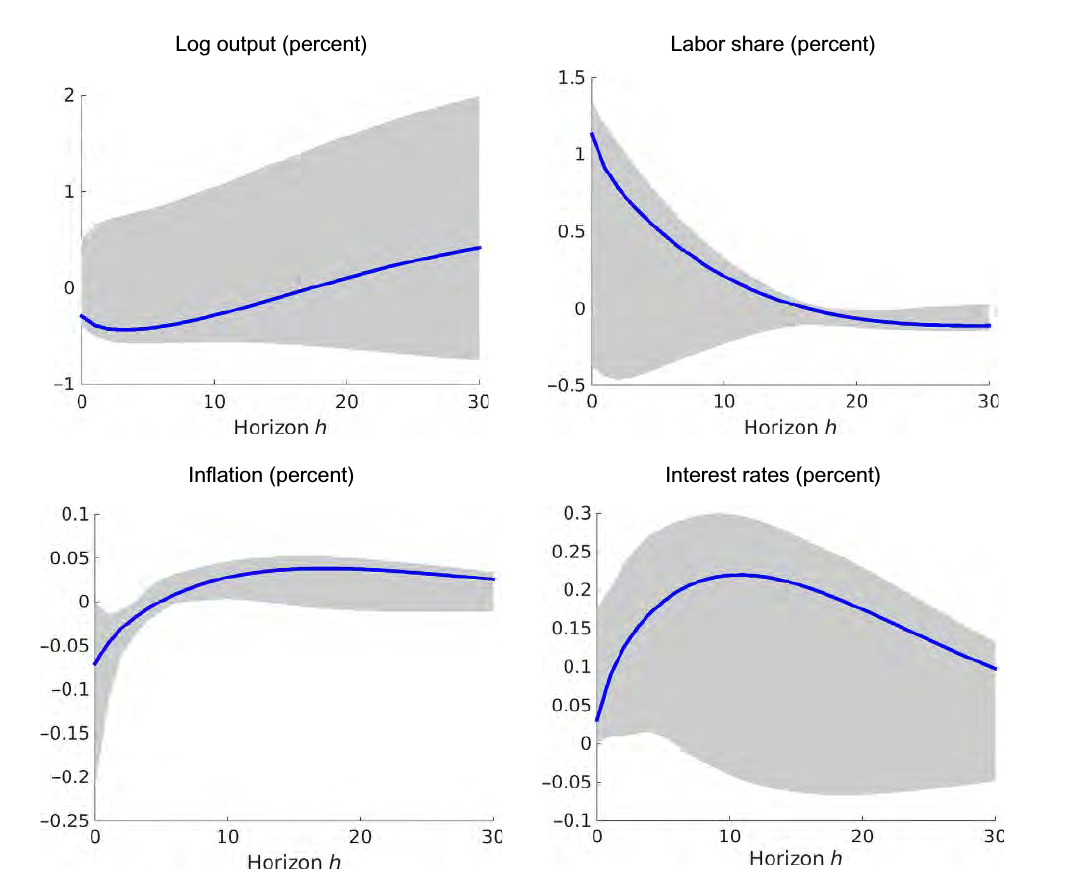
\includegraphics[width=12cm]{./Figures/20180409-irfs-var}
  \label{fig:stylized-ssrep-irfs-var}
%
%  \small{}
\end{figure}

如图\ref{fig:stylized-ssrep-irfs-var}所示,$t=0$时刻货币政策的点冲击,在随后$t+h$时刻产出增速、劳动收入份额、通货膨胀率、利率的已识别响应的区间用阴影表示。需要指出的是,4个状态变量的响应区间不同,尤其是产出增速和劳动收入份额的响应符号(方向)不够清晰,这是由于模拟过程中注入到系统里的货币政策冲击的符号限定不够强。

\subsection{条件矩的限制}
\label{sec:stylized-ssrep-empirics-moments}
根据DSGE模型的均衡条件,可以推得一组条件矩限制(第\ref{sec:stylized-ssrep-restrictions}节),这组条件矩限制是基于全体的理想状况给出的;基于实际观测到的抽样样本的平均数,可以对全体矩限制作样本矩限制的近似。但需要指出的是,这组近似矩并不是完全无条件的,例如NKPC得到的矩\eqref{eq:stylized-sspre-moment-nkpc-info-set}中含有隐含变量——当期价格加成的冲击$\lambda_{t}$,从而使得进一步从事矩分析变得困难。

对全体矩限制的样本近似常常采用广义矩估计法(generalized method of moments, GMM)\index{generalized method of moments (GMM) \dotfill 广义矩估计法},我们将在随后进一步介绍。\todo{敲进键盘之后,做一个ref}%Sec 11.4。

\section{处理趋势}
\label{sec:stylized-ssrep-empirics-trends}
趋势(trend)是宏观经济时间序列数据的一个重要特征。在第\ref{sec:stylized-dsge-model}节典型DSGE模型的设定中,就含有了这样一种随机趋势,它由生产率过程$\log Z_{t}$产生,表现为一个含有漂移的随机游走。尽管生产率中的趋势导致模型中的其他变量如消费、产出、实际工资等也含有趋势,但根据这样的模型设定,消费产出比、劳动收入份额等都应当是平稳的。

然而实际观察到的经济数据与模型的假设不符,如图  \ref{fig:stylized-ssrep-empirics-ratio-yl-cy}所示,1996-2015年间中国的这两组数据并不平稳。实际观测数据中含有的趋势并未反映在DSGE模型中,导致观测数据和模拟数据之间产生了一阶不一致。
\begin{figure}[htbp]
  \caption{中国的劳动收入份额和消费产出比}\small{数据来源:中国统计年鉴。}
  \centering
  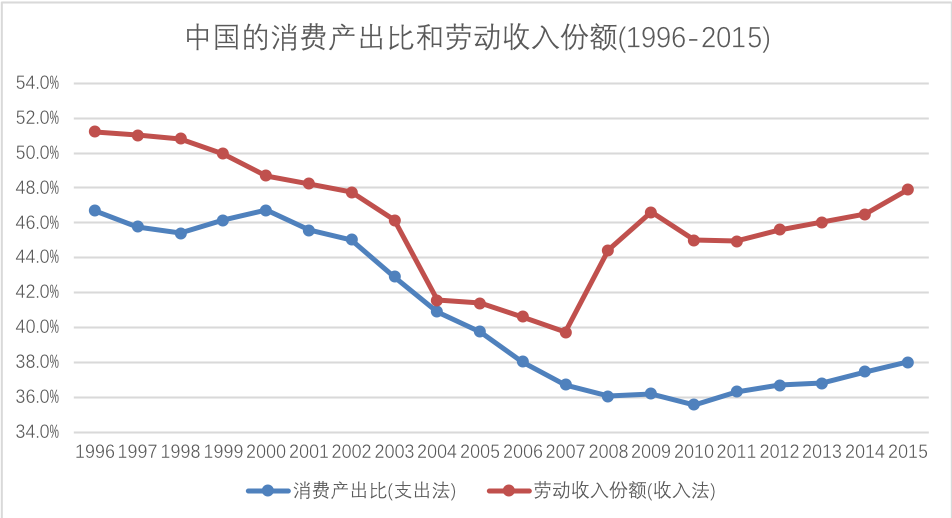
\includegraphics[width=12cm]{./Figures/20180409-ratio-yl-cy}
  \label{fig:stylized-ssrep-empirics-ratio-yl-cy}
%
%  \small{}
\end{figure}

大多数DSGE模型在实际应用过程中都暗含着反事实趋势,这是由于模型中往往包含一些共趋势(co-trending)的限制条件\citep{Hatanaka:2012bo},例如一条最的平衡增长路径(alanced growth path, BGP),根据这样的路径设定,模型假定
\begin{itemize}
  \item 产出、消费、投资、资本存量、实际工资等经济变量表现出相同的运动趋势,
  \item 资本回报率平稳。
\end{itemize}
这些假设条件,或多或少都与实际观测到的数据不匹配。

经济学家已提出许多种方法,致力于缩小两组数据之间的不匹配,如
\begin{enumerate}
  \item 对观测到的每一个变量时间序列分别作去适宜的去趋势处理,进而比较(去趋势后的)观测数据与模拟数据;
  \item 用同一种趋势滤波对观测数据和模拟数据作处理,进而比较;
  \item 构建混合模型,如\cite{Canova:2014be}模型一方面含有灵活的非结构性的趋势成分,另一方面利用结构DSGE模型取描述围绕缩减式趋势的上下波动;
  \item 将更多现实中的趋势直接引入到DSGE模型的结构中。
\end{enumerate}

从宏观经济学研究的角度上来说,这4种方法中,越是接近方法4,就越值得提倡。
